% !TeX spellcheck = it_IT
\section{Cosa sono i Bitcoin?}

Bitcoin è una valuta elettronica creata nel 2008 da Satoshi Nakamoto, uno pseudonimo dietro al quale non si sa ancora con la precisione chi si nasconde.
Con il termine Bitcoin viene denotata sia la rete che consente il possesso e il trasferimento di denaro, sia la moneta. Per convenzione, Bitcoin si riferisce alla tecnologia della rete, mentre \textit{bitcoin} alla valuta stessa.

Come ogni valuta, i bitcoin possono essere trasferiti tramite gli utenti, grazie ad un protocollo che viene rispettato all'interno della rete Internet, il quale può essere eseguito su differenti dispositivi, in modo tale da permettere la fruibilità del servizio anche attraverso gli smartphones.
 
I bitcoins possono essere comprati, venduti e scambiati con altre valute, tramite degli organismi specializzati nel cambio di monete virtuali. In un certo senso, Bitcoin è la forma perfetta di denaro per Internet, dal momento che è estremamente veloce, sicuro e senza limiti.

A differenza delle altre valute, i bitcoin sono esclusivamente virtuali, dietro di essi non esistono monete fisiche. Tali bitcoin vengono coinvolti in transazioni da mittente a ricevente, i quali possiedono delle chiavi crittografiche pubbliche e private che servono per trasmettere e sbloccare la spesa dei bitcoin ricevuti.
Infatti, senza la chiave privata, chi riceve i bitcoin non può spenderli in nessun modo. Tali chiavi vengono conservate all'interno di un \textit{wallet}, letteralmente un "portafoglio". Ogni wallet è caratterizzato da un indirizzo Bitcoin il quale è univoco e ha la funzione di fare riferimento ad uno dei partecipanti alla transazione. In questo modo, quando viene effettuato uno scambio di bitcoin, vengono visualizzati solamente gli indirizzi dei wallet. Questa caratteristica permette quindi di rendere anonime le transazioni, dato che agli indirizzi non è connesso in nessun modo il nome o il cognome dell'individuo o dell'associazione che interviene nello scambio.

La rete Bitcoin, oltre ad essere completamente virtuale, è priva di un'unità centralizzata, infatti essa è costituita da un sistema distribuito peer-to-peer.\\
I bitcoin vengono creati tramite un processo, detto \textit{mining}, che permette a chiunque di mettersi in competizione per trovare una soluzione ad un problema matematico. Ogni persona che partecipa alla rete bitcoin, potrebbe operare come un \textit{miner}, ovvero colui che cerca di risolvere il problema matematico per generare bitcoin, usando le capacità del proprio computer messo a disposizione della computazione.\\

Quando viene effettuato uno scambio di bitcoin tra due o più wallet, viene creata una \textit{transazione}. Ogni transazione viene conservata in una struttura dati chiamata \textbf{blocco}, il quale a sua volta va a costituire la \textbf{Blockchain}.

\section{Cos'è la Blockchain?}
La Blockchain, letteralmente \textit{catena di blocchi}, è una base di dati distribuita, che permette la memorizzazione delle transazioni raggruppate in blocchi connessi tra loro, ognuno con il suo successivo. Ogni blocco è una struttura dati che contiene un numero variabile di transazioni, inserite dal \textit{miner} che ha minato il blocco, fino ad un tetto massimo di 1MB per singolo blocco.\\

L'idea di base della Blockchain, deriva dal concetto di \textbf{libro mastro}, il registro della contabilità in cui sono riuniti tutti i conti che compongono un dato sistema contabile. In questo caso il sistema contabile sarebbe la rete Bitcoin, mentre la Blockchain sarebbe il libro mastro che contiene tutti i conti, ovvero le transazioni. \\

L'antico libro mastro, veniva utilizzato come fonte ufficiale per la memorizzazione degli scambi e dei passaggi di proprietà. Infatti, quando veniva fatta una compravendita tra mittente e ricevente, veniva controllato sul libro mastro se il ricevente non avesse speso precedentemente il denaro, e se il mittente non avesse già venduto la merce usata nello scambio.

Infine, se fosse andato tutto a buon fine, veniva registrata la transazione sul libro mastro, in modo da essere consultabile e pubblica per le successive transazioni.

Un principio importante di questo meccanismo è la fiducia, la quale tutti ripongono nel libro mastro: ognuno si fida del gestore della memorizzazione delle transazioni, al punto che, chi compra e chi vende, può effettuare scambi anche senza fidarsi reciprocamente. Quindi, il libro mastro è una garanzia, sia per il mittente che per il ricevente dello scambio. Inoltre, le banche possono perciò controllare gli scambi che vengono fatti e il denaro posseduto da ogni partecipante alle transazioni.

La Blockchain, come già sottolineato, è una struttura dati composta da diverse unità di base, dette blocchi. Infatti, blockchain significa letteralmente \textit{catena di blocchi}.

Quindi, tali blocchi vengono "incatenati", ovvero collegati tra loro tramite un protocollo ben definito nella struttura del sistema bitcoin. 

Ogni blocco all'interno della blockchain, è identificato da un codice hash, generato applicando l'algoritmo di crittografia SHA256 all'header del blocco. Un singolo blocco è collegato al suo predecessore, conosciuto come "blocco genitore", attraverso il campo \textit{previous block hash} all'interno del proprio header. In altre parole, ogni blocco contiene l'hash del proprio blocco genitore all'interno dell'header. Infine, la sequenza dei vari hash genera una catena che collega tutti i blocchi all'indietro, fino al blocco numero zero.

\subsection{Mining}

Le monete bitcoin sono "coniate" durante la creazione di ciascun blocco ad un tasso fisso. Ogni blocco, generato all'incirca ogni 10 minuti, contiene nuovi bitcoin, creati da zero.
Il \textit{mining} inoltre serve per proteggere il sistema bitcoin contro transazioni fraudolente o transazioni che cercano di spendere lo stesso numero di bitcoin più di una volta, problema conosciuto con il nome di \textit{double-spend} (doppia-spesa).

I miner validano le transazioni e le registrano sul \textit{ledger} globale, ovvero la Blockchain, creando un nuovo blocco e inserendo le transazioni al suo interno, per poi aggiungere il blocco alla catena. Perciò, i miner raccolgono un certo numero di transazioni e cercano di inserirle all'interno di un nuovo blocco creato appositamente. Tutte le transazioni che poi risultano alla fine all'interno di tale blocco, sono considerate \textit{confirmed} (ovvero confermate), ovvero una sorta di etichetta che permette al ricevente di tali bitcoin di spenderli successivamente.

Lo scopo dei miner è quello di guadagnare bitcoin, e possono ottenerli in due modi: 
\begin{itemize}
	\item quando un nuovo blocco viene aggiunto alla Blockchain, si ottiene un premio in bitcoin
	\item per ogni transazione vengono pagate le \textit{fees} (=tasse) al miner
\end{itemize}

Al fine di ottenere il premio, i miner devono trovare la soluzione ad un problema matematico molto difficile basato su un algoritmo di crittografia. La soluzione a tale problema, chiamata \textbf{proof of work}, è inclusa all'interno del nuovo blocco, e serve come prova che il miner ha impiegato un notevole sforzo di elaborazione. La competizione tra i miner per trovare la proof of work per guadagnare bitcoin è alla base della sicurezza del sistema Bitcoin.

Il processo della generazione di nuove monete è chiamato \textbf{mining} perchè la ricompensa è progettata in modo da simulare rendimenti decrescenti, esattamente come l'estrazione di metallo prezioso.
La fornitura di valuta bitcoin è creata attraverso il mining, analogamente alla procedura con cui una banca centrale crea moneta stampando banconote. 

L'ammontare del premio del mining a Gennaio 2009 era di 50 bitcoin per blocco e a Novembre 2012 già si era dimezzato fino ad ottenere 25 bitcoin. Attualmente il guadagno del premio del mining risulta 12.5 bitcoin per blocco.
Seguendo questo processo, il premio per il mining di un blocco, decrescerà esponenzialmente fino all'anno 2140, quando tutti i bitcoin (20.9999998 milioni) saranno emessi. All'incirca dopo il 2140 non saranno più prodotti nuovi bitcoin e il miner andrà a guadagnare solamente tramite le tasse applicate per ogni transazione.

I miners guadagnano bitcoin per ogni transazione tramite le tasse. Esse vengono calcolate come eccesso di bitcoin tra le transazioni di input e quelle di output.



\subsection{Blockchain Forks}

Dal momento che la Blockchain è una struttura dati decentralizzata, copie differenti non sono sempre consistenti. Infatti, i blocchi possono arrivare a nodi diversi in tempi diversi, creando differenti rami all'interno della stessa blockchain.

Sebbene un blocco abbia solo un genitore, esso può avere temporaneamente un diverso numero di figli. Ogni figlio si riferisce allo stesso blocco genitore e contiene lo stesso hash del genitore nel campo  \textit{previous block hash}. Questa temporanea molteplicità di figli può causare una \textit{fork} (letteralmente \textit{biforcazione}), ovvero una situazione in cui blocchi differenti vengono creati quasi simultaneamente da diversi miners.

Per risolvere il problema della biforcazione, ogni nodo Bitcoin seleziona sempre e cerca di estendere la catena di blocchi che soddisfa il sistema \textit{proof-of-work}.


%By summing the difficulty recorded in each block in a chain, a node can calculate the total amount
%of proof of work that has been expended to create that chain. As long as all nodes select
%the longest cumulative difficulty chain, the global bitcoin network eventually converges
%to a consistent state. Forks occur as temporary inconsistencies between versions of the
%blockchain, which are resolved by eventual reconvergence as more blocks are added to
%one of the forks.

\begin{figure}[htbp]
	\centering%
	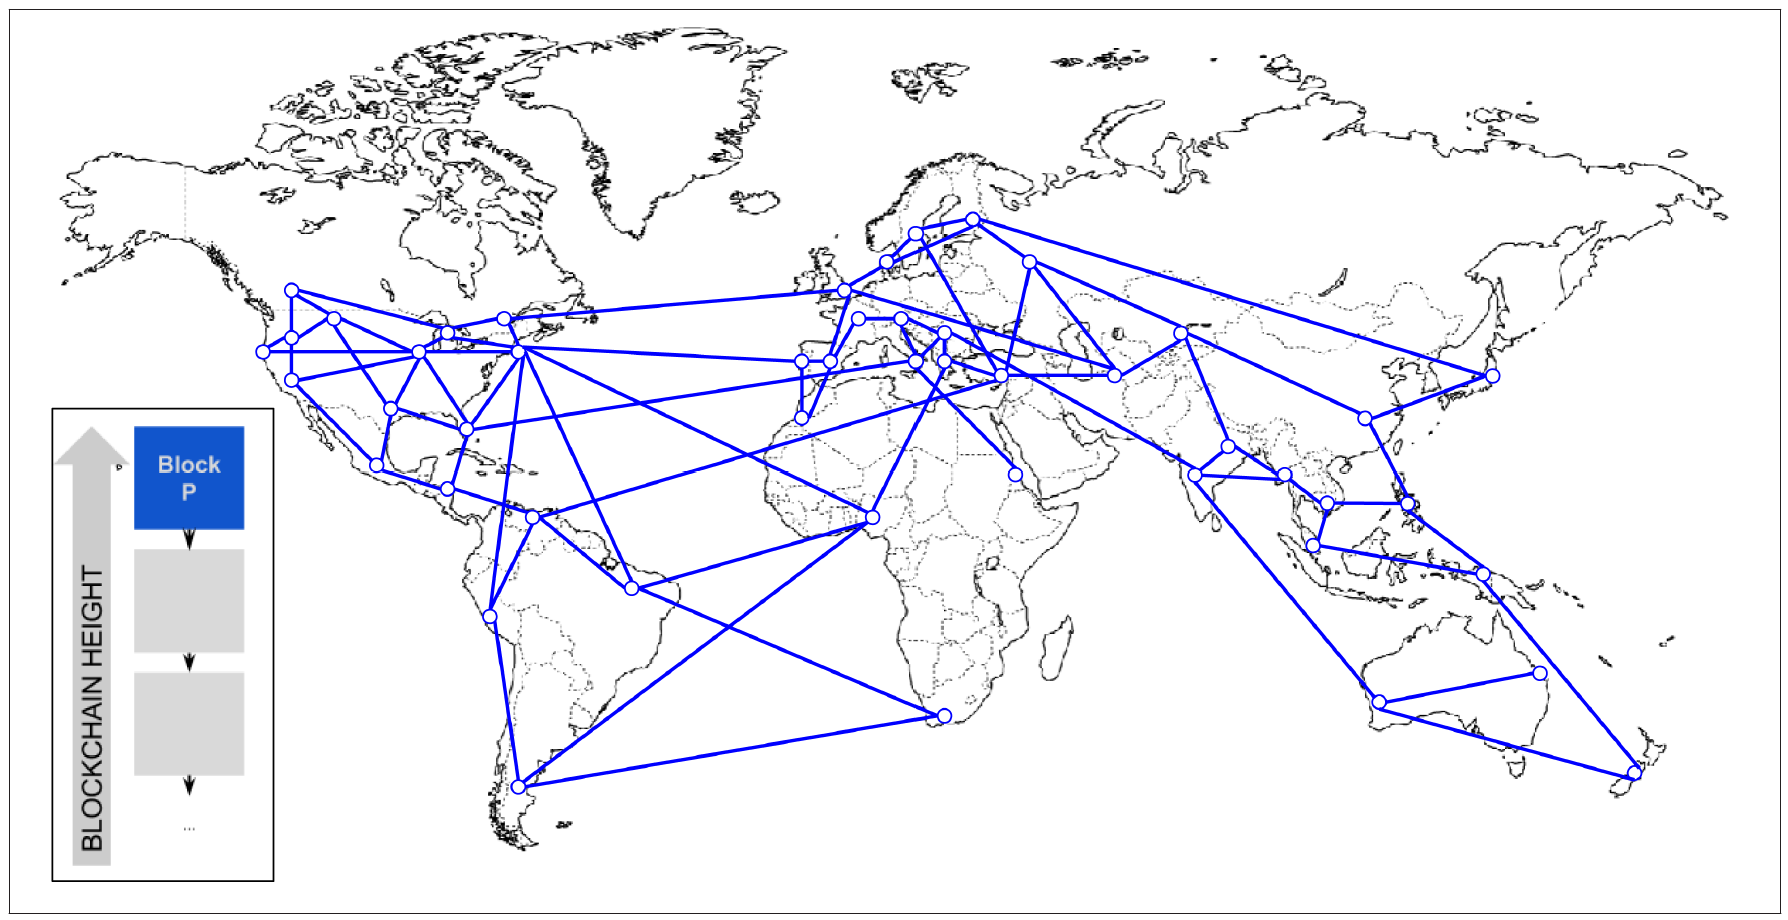
\includegraphics[width= 0.8 \linewidth]{figure/fork1}

	\caption{Fork - parte 1\label{fig:sottofigure}}
\end{figure}



%	Minare bitcoin
%		come si fa x
%		chi lo fa x
%		guadagno x
%		complessità computazionale
%		merkle hash tree
	

\section{Le Transazioni}

Come è stato detto in precedenza, una transazione è uno scambio di monete bitcoin tra due o più individui. Per esempio, se Alice vuole dare 1BTC a Bob, ha bisogno di effettuare una transazione inserendo come input l'importo da trasferire e l'indirizzo del wallet di Bob. \\ 

Nella maggior parte dei casi, la quantità di denaro che partecipa alla transazione non è quasi mai
Secondo la configurazione predefinita dal protocollo, quando viene effettuata una transazione che non implica la spesa dell'intero importo contenuto nel wallet del mittente, è previsto che venga creata un ulteriore transazione con il 

Una caratteristica delle transazioni è che possono partecipare più wallet contemporaneamente: ad esempio, un individuo può inviare con la stessa transazione, una quantità di bitcoin a due individui diversi, in modo da recapitare ciascuno la quantità di bitcoin desiderata. 

\section{Grafo delle transazioni}
\section{Caratteristiche del grafo}